\documentclass[conference]{IEEEtran}
\usepackage{cite}
\usepackage{amsmath,amssymb}
\usepackage{graphicx}
\usepackage{booktabs}
\usepackage{url}
\graphicspath{{figures/}}

\begin{document}

\title{Analysis and Extension of a Game Theory Model for Multi-Robot Cooperation in Industry 4.0}

\author{
\IEEEauthorblockN{Sneha Shendre}
\IEEEauthorblockA{Engineering Physics, SVNIT Surat\\ \texttt{<roll no.>}}
\and
\IEEEauthorblockN{<Member 2>}
\IEEEauthorblockA{<Department>, SVNIT Surat\\ \texttt{<roll no.>}}
\and
\IEEEauthorblockN{<Member 3>}
\IEEEauthorblockA{<Department>, SVNIT Surat\\ \texttt{<roll no.>}}
}

\maketitle

\begin{abstract}
We study the paper by Gindullina \emph{et al.}~\cite{paper}, which models a scanning robot and a robotic arm in a factory as players in a $2\times2$ game and in a Bayesian game. We first reproduce all of the paper's tables and equilibria in Python. We then analyse the results. The equilibrium $(D,C)$ is both Pareto-dominant and risk-dominant, and the constant $P$ decides how many equilibria exist. Surprisingly, the paper's Bayesian equilibria always achieve coordination, which contradicts its conclusion. Simulating fictitious play, the robots reach $(D,C)$ in 90\% of runs. Finally, we propose an extension in which the item's real defect status matters and the arm sees the scan result. Solved by backward induction, it gives behaviour that the paper only assumes, such as moving rejected items fast.
\end{abstract}

\begin{IEEEkeywords}
Nash equilibrium, Bayesian games, fictitious play, backward induction, multi-robot systems
\end{IEEEkeywords}

\section{Introduction}
Robots in modern factories have to work together without a central controller, and game theory is a natural tool for this~\cite{tadelis}. The paper we chose~\cite{paper} looks at a quality-control station with two robots. A scanner $S$ chooses a detailed scan ($D$) or a quick scan ($Q$). An arm $A$ moves the item fast ($F$) or cautiously ($C$). The pairs $(D,C)$ and $(Q,F)$ are called \emph{coherent} and give a higher reward.

Our goals were to (1) check the paper's results by coding them, (2) analyse what the results mean, (3) see what happens when the game is played repeatedly, and (4) fix a limitation we noticed: the payoffs never depend on whether the item is actually defective.

\section{The Paper's Model}
Each robot's payoff is
\begin{equation}
u = P\cdot r - c_i + b_i,
\end{equation}
where $c_i$ is the cost of the action and $b_i$ is a bonus for the safer action. The reward is $r=1$ for a coherent pair and $r=0.5$ otherwise, and $P=10$. The values from Table~I of the paper are $c_D=2, c_Q=1, c_F=1, c_C=2$ and $b_D=1, b_Q=-1, b_F=-1, b_C=1$. Fig.~\ref{fig:std} shows the resulting game.

In the Bayesian version, the scanner is ``mistaken'' with probability $p$ and the arm with probability $q$. If both robots are of the same type (both mistaken or both right), the normal table is used. If only one is mistaken, the coherent pairs flip to $(D,F)$ and $(Q,C)$. Each robot's strategy is a plan with one action per type, e.g.\ $DQ$.

\begin{figure}[t]
\centering
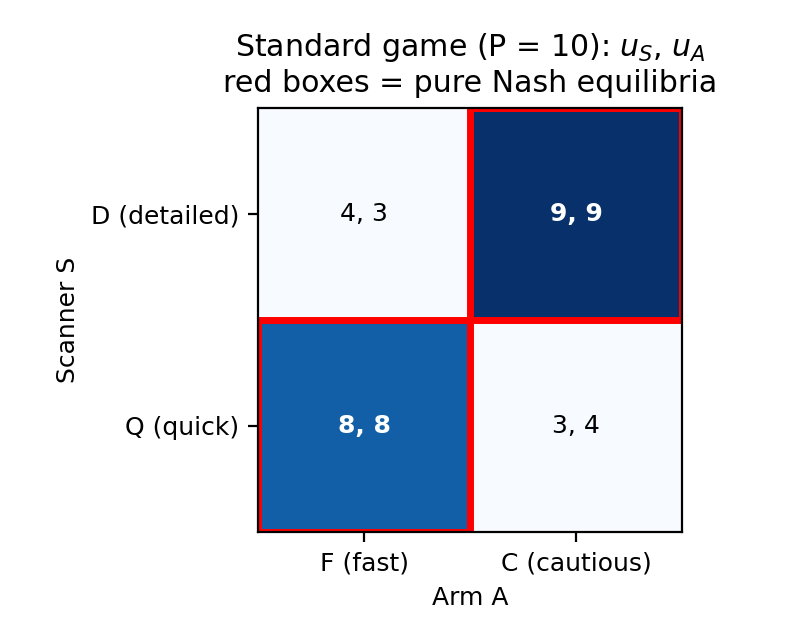
\includegraphics[width=0.8\columnwidth]{fig1_standard_game}
\caption{The standard game with $P=10$. Red boxes are the pure Nash equilibria.}
\label{fig:std}
\end{figure}

\section{Reproducing the Paper}
We wrote the model in Python (\texttt{paper\_game.py}). To find pure Nash equilibria we check every cell of the table, asking whether either player can gain by switching. For the mixed equilibrium we use the indifference method~\cite{tadelis}. For the Bayesian game we compute the expected payoff of every pair of plans over the four type combinations.

All our numbers match the paper. We get Table~III, the pure equilibria $(D,C)$ and $(Q,F)$, and the mixed equilibrium $\Pr[D]=2/5$, $\Pr[F]=3/5$ (Fig.~\ref{fig:br}). We also get all 32 values of Table~VII and the Bayesian equilibria $(DQ,CF)$ and $(QD,FC)$ (Fig.~\ref{fig:bayes}). These checks are written as automated tests in \texttt{test\_project.py}.

The paper never says which letter of a plan belongs to which type. By matching Table~VII we found that the first letter is the action when the robot is mistaken, and the second when it is right. We also found two small typos. Table~VI is stated for $p=q$ but one entry is written as $4q+4$; it should be $4p+4$. The best responses are labelled $BR_S$ although they are the arm's best responses.

\begin{figure}[t]
\centering
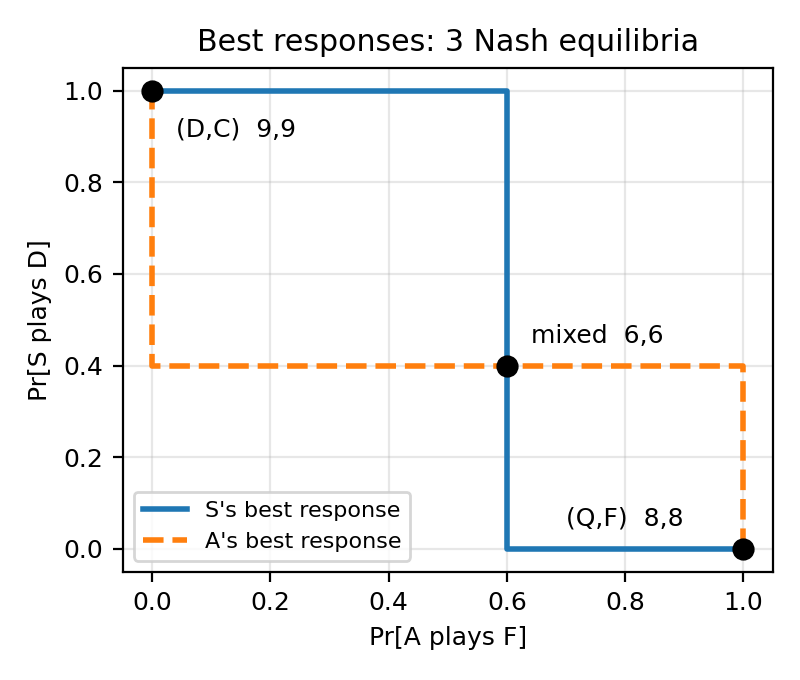
\includegraphics[width=0.8\columnwidth]{fig2_best_response}
\caption{Best-response curves. They cross at three points: two pure equilibria and one mixed equilibrium.}
\label{fig:br}
\end{figure}

\begin{figure}[t]
\centering
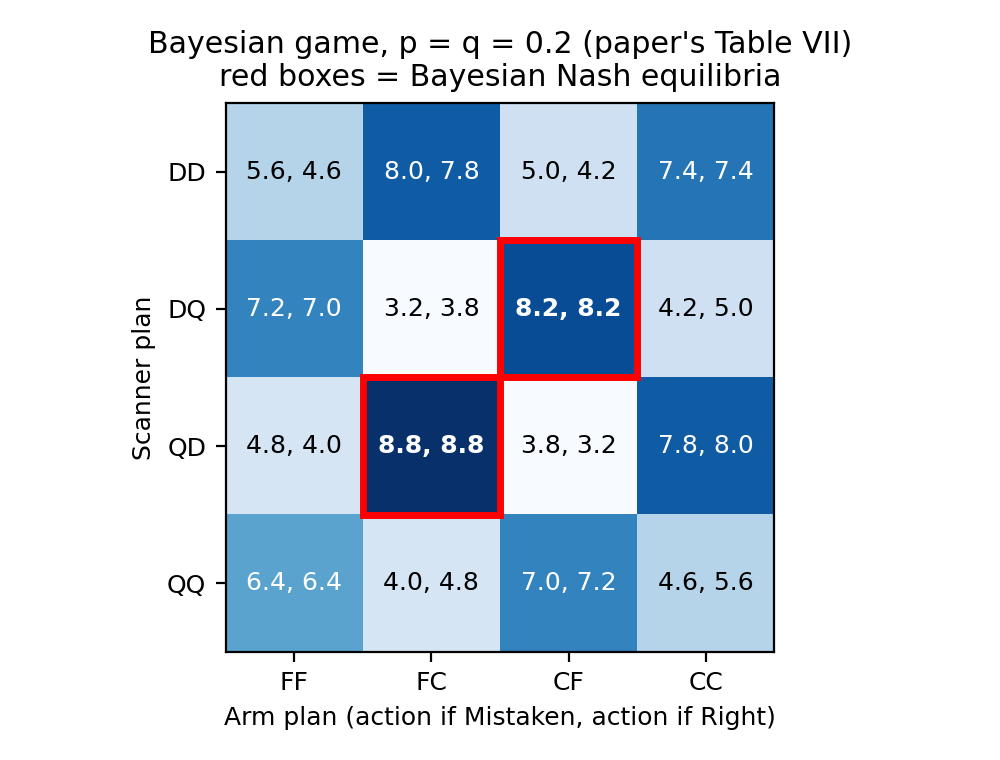
\includegraphics[width=0.9\columnwidth]{fig3_bayesian_table}
\caption{Our reproduction of the paper's Table~VII ($p=q=0.2$). Red boxes are the Bayesian Nash equilibria.}
\label{fig:bayes}
\end{figure}

\section{Analysis}
\subsection{Which equilibrium will the robots pick?}
The paper says that having several equilibria means the system has no single operating point. However, $(D,C)$ is better than $(Q,F)$ in two standard ways:
\begin{itemize}
\item \textbf{Pareto dominance:} both robots get more at $(D,C)$ (9, 9) than at $(Q,F)$ (8, 8).
\item \textbf{Risk dominance}~\cite{harsanyiselten}: at $(D,C)$ each robot loses $9-3=6$ by switching alone, giving a product of 36. At $(Q,F)$ the product is $4\times4=16$. So $(D,C)$ is also the ``safer'' equilibrium.
\end{itemize}
The mixed equilibrium gives only 6 to each robot, which is worse than both pure equilibria.

\subsection{The constant $P$ is not just a normalisation}
The paper calls $P$ ``just a normalization constant''. But the mixed equilibrium $\Pr[D]=(P-2)/2P$ only makes sense when $P>2$. For $P<2$ the reward for coordinating is too small, $D$ and $C$ become dominant strategies, and $(D,C)$ is the only equilibrium. We confirmed this in our tests with $P=1.5$. So $P$ decides whether the robots face a coordination problem at all.

\subsection{The Bayesian equilibria always coordinate}
The paper concludes that mistakes ``can steer the equilibrium away from using a coherent strategy''. We computed the probability that the robots actually receive the coherent reward in each equilibrium. For both $(DQ,CF)$ and $(QD,FC)$ it is exactly 1, for every $p$ and $q$ we tried.

The reason is the model itself. In a Bayesian game each player knows its own type~\cite{harsanyi}, so here a robot \emph{knows} when it is mistaken and simply corrects for it. A more realistic model would let robots know only a noisy measurement, not whether they are wrong.

The paper also only studies $p=q$. Fig.~\ref{fig:pq} shows all $(p,q)$: the same two equilibria exist everywhere, and $(DD,CC)$ is an extra equilibrium when both $p$ and $q$ are between 0.4 and 0.6.

\begin{figure}[t]
\centering
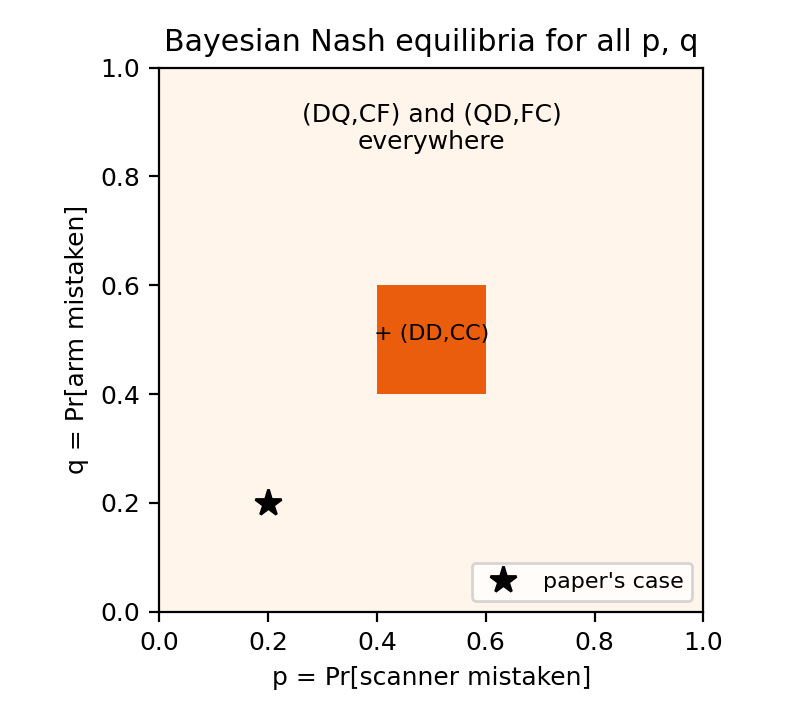
\includegraphics[width=0.75\columnwidth]{fig4_bayesian_pq_map}
\caption{Bayesian Nash equilibria for all values of $p$ and $q$.}
\label{fig:pq}
\end{figure}

\subsection{Limitations of the model}
The paper's text explains the robots' choices using the item: defective items should be moved fast, complex items need careful handling. However, these facts never enter the payoff formula. In addition, the error probability is the same for detailed and quick scans, so a detailed scan is not actually more accurate. Finally, the robots move at the same time, although in a real factory the arm moves after the scan.

\section{Repeated Play: Fictitious Play}
The paper claims that the equilibrium is a ``point of convergence'' for the robots, but it does not show how they would get there. We simulated fictitious play~\cite{brown,fudenberg} (\texttt{learning.py}). In each round, each robot plays a best response to how often the other robot has used each action so far. Starting beliefs are random.

In all 100 runs the robots settled on a pure equilibrium: 90\% at $(D,C)$ and 10\% at $(Q,F)$ (Fig.~\ref{fig:fp}). This supports the paper's claim, and it also shows that $(D,C)$ is the much more likely outcome.

\begin{figure}[t]
\centering
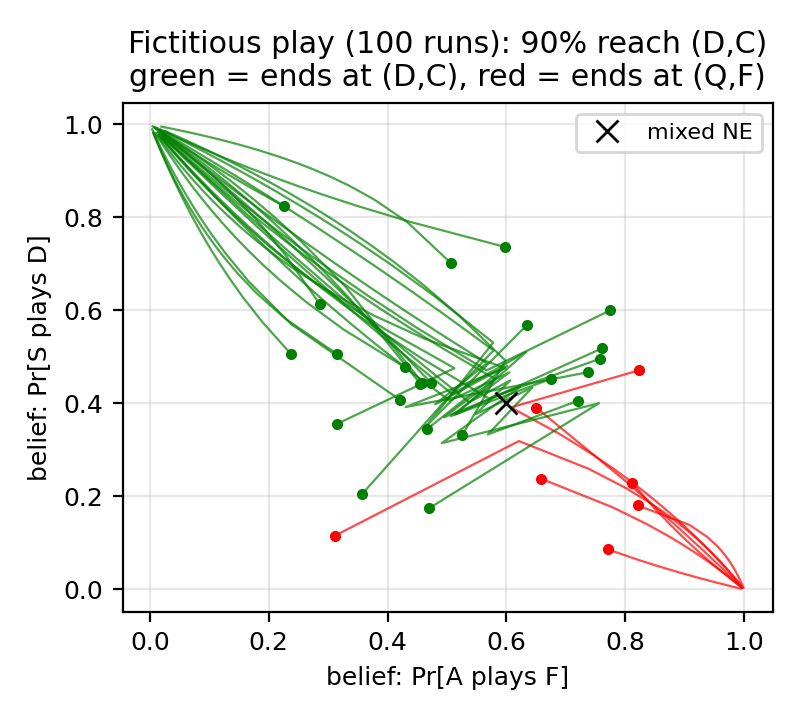
\includegraphics[width=0.8\columnwidth]{fig5_fictitious_play}
\caption{Fictitious play from 30 random starts (green: ends at $(D,C)$, red: ends at $(Q,F)$).}
\label{fig:fp}
\end{figure}

\section{Our Extension: A Defect-Aware Inspection Game}
To fix the limitations above, we built a new game (\texttt{defect\_game.py}):
\begin{enumerate}
\item Nature decides if the item is defective, with probability $\rho$. Both robots can see whether the item is simple or complex.
\item The scanner chooses $D$ or $Q$. A detailed scan detects more defects, and a quick scan is especially bad on complex items (55\% detection instead of 95\%).
\item The scan gives a verdict, \emph{pass} or \emph{fail}.
\item The arm \textbf{sees the verdict} and chooses $F$ or $C$. Fast moves break complex items more often.
\end{enumerate}
Losses are 30 for shipping a defective item, 5 for rejecting a good one, and 20 for breaking a good item that is being shipped. Breaking a rejected good item costs only 2, since it is checked again anyway. Action costs are the same as in the paper. Each robot cares fully about its own job and half about the other robot's job. All these numbers are our own assumptions.

Since the arm moves after the scanner, we solve the game by \textbf{backward induction}~\cite{tadelis}. First we find the arm's best move for each verdict, using Bayes' rule for the probability that the item is good. Then the scanner picks the scan mode that is best for it, knowing how the arm will react.

\textbf{Results.} Three behaviours appear without being assumed:
\begin{itemize}
\item Rejected items are always moved fast. This is exactly the intuition in the paper, but here it comes out of the model.
\item Items that pass are moved cautiously if complex and fast if simple.
\item The scanner uses a detailed scan only when defects are common enough: above $\rho\approx0.06$ for complex items and $\rho\approx0.38$ for simple items (Fig.~\ref{fig:scan}).
\end{itemize}
For complex items with few defects, the best plan is a quick scan followed by cautious handling. The paper would call this pair ``not coherent'', yet here it is the best choice.

Fig.~\ref{fig:loss} compares our equilibrium with the paper's two coherent pairs used for every item. For simple items, our equilibrium has up to 38\% lower loss than always using $(D,C)$. For complex items, always using $(Q,F)$ loses 1.6 to 2.4 times more. Compared with the better of the two fixed pairs for each item type, our equilibrium saves up to 7\% on simple items and up to 15\% on complex items.

\begin{figure*}[t]
\centering
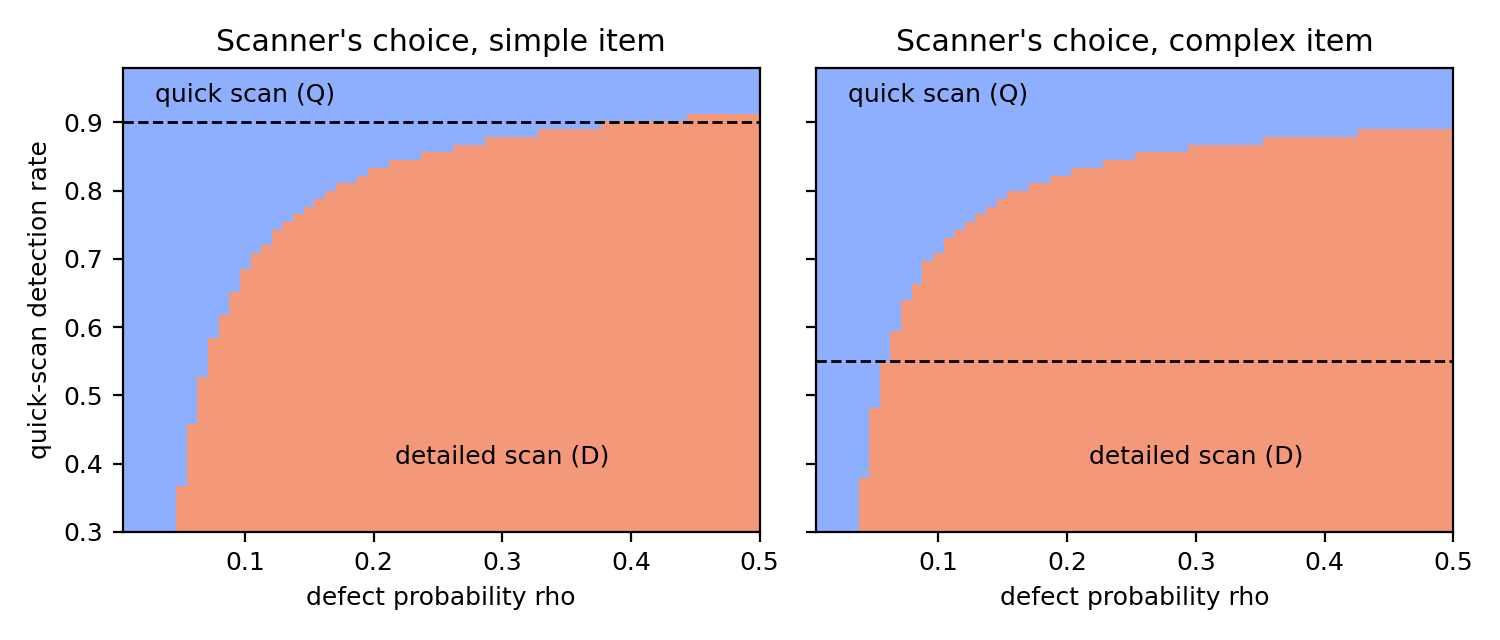
\includegraphics[width=0.8\textwidth]{fig6_extension_scan_choice}
\caption{Extension: the scanner's choice for different defect probabilities and quick-scan accuracies. The dashed line is our default accuracy.}
\label{fig:scan}
\end{figure*}

\begin{figure*}[t]
\centering
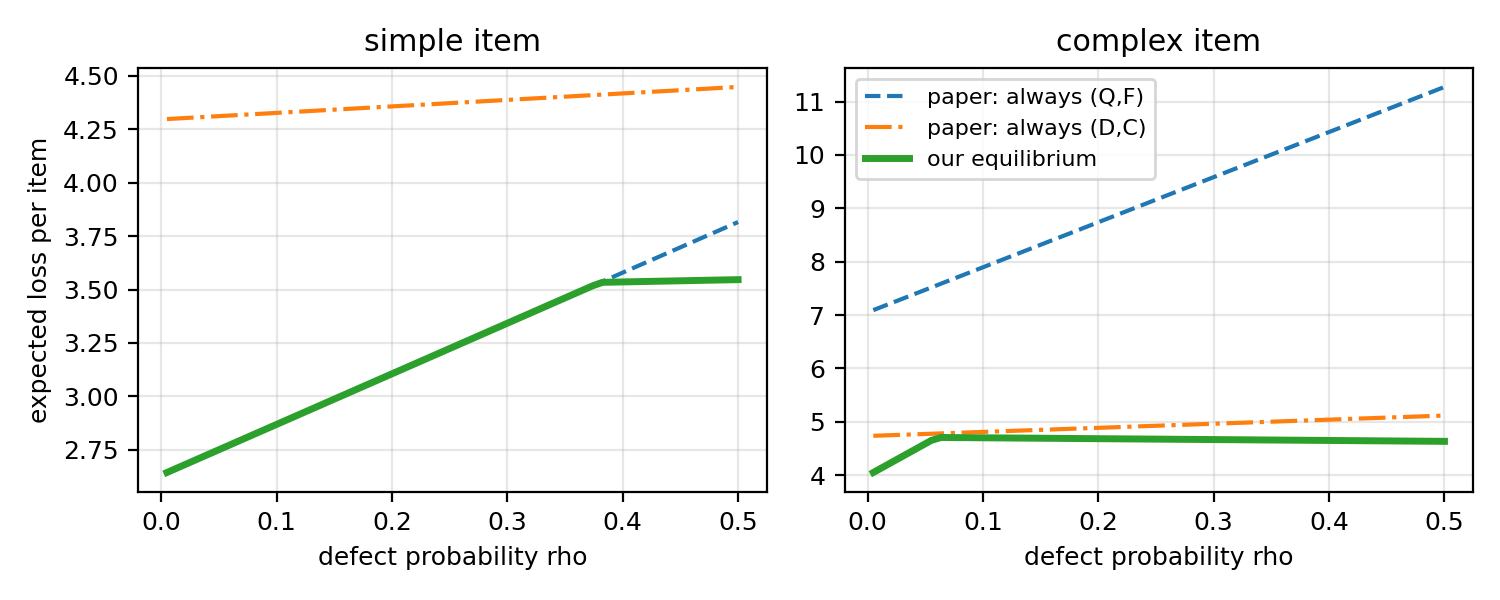
\includegraphics[width=0.8\textwidth]{fig7_extension_vs_paper}
\caption{Extension: expected loss per item of our equilibrium compared with the paper's coherent pairs used for every item.}
\label{fig:loss}
\end{figure*}

\section{Conclusion}
We reproduced all results of~\cite{paper} and found that its main conclusions need some correction. $(D,C)$ is the clear choice by Pareto dominance, risk dominance and fictitious play. $P$ controls whether the game is a coordination problem at all. The Bayesian equilibria never actually fail to coordinate, because the robots know their own mistakes.

Our extension adds the real defect status and lets the arm see the scan result. As a result, behaviours the paper only assumes appear naturally, and losses drop compared with the paper's fixed strategies.

Future work could use real detection and breakage rates, let robots know only noisy measurements, and study what happens when the robots' goals are less aligned.

\section*{Code}
All code, figures and tests are available at \url{https://github.com/<username>/gt-project}.

\begin{thebibliography}{00}
\bibitem{paper} E. Gindullina, E. Peagno, G. Peron, and L. Badia, ``A game theory model for multi robot cooperation in Industry 4.0 scenarios,'' in \emph{Proc. IEEE Asia Pacific Conf. Circuits Syst. (APCCAS)}, 2021.
\bibitem{tadelis} S. Tadelis, \emph{Game Theory: An Introduction}. Princeton, NJ, USA: Princeton Univ. Press, 2013.
\bibitem{harsanyi} J. C. Harsanyi, ``Games with incomplete information played by `Bayesian' players, Part I,'' \emph{Manage. Sci.}, vol. 14, no. 3, pp. 159--182, 1967.
\bibitem{harsanyiselten} J. C. Harsanyi and R. Selten, \emph{A General Theory of Equilibrium Selection in Games}. Cambridge, MA, USA: MIT Press, 1988.
\bibitem{brown} G. W. Brown, ``Iterative solution of games by fictitious play,'' in \emph{Activity Analysis of Production and Allocation}, T. C. Koopmans, Ed. New York, NY, USA: Wiley, 1951, pp. 374--376.
\bibitem{fudenberg} D. Fudenberg and D. K. Levine, \emph{The Theory of Learning in Games}. Cambridge, MA, USA: MIT Press, 1998.
\end{thebibliography}

\end{document}
